%! Licence = CC BY-NC-SA 4.0

%! Author = gianfluetsch
%! Date = 22. Jan 2022
%! Project = icth_summary

\section{Leitungscodierung}
\subsection{Rinkel}
\subsubsection{Prüfung FS2009}
Ein NRZ Signal hat den unten aufgezeichneten Signalverlauf. Skizzieren Sie den entsprechenden Signalverlauf sowohl für den Manchester Code als auch für den AMI-Code.
\begin{center}
    \vspace{-8pt}
    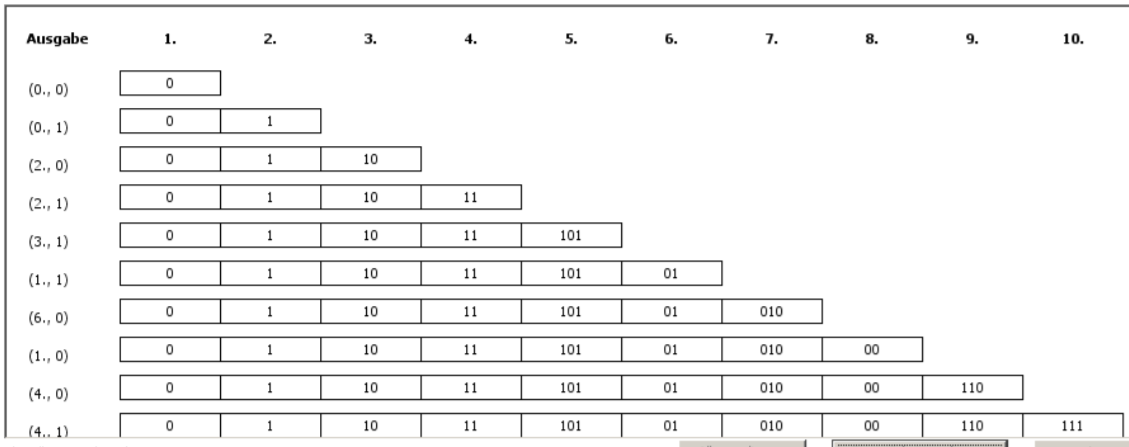
\includegraphics[width=.8\linewidth]{./06-leitungscodierung/fs2009}
    \vspace{-8pt}
\end{center}

Vergleichen Sie die drei Codierungsarten anhand der oben gegebenen und der erstellten Codierungen.\\
\textit{Lange 0Folgen werden beim AMI Code zu einem Problem wegen der Phasen und Taktrückgewinnung. NRZ hat dieselben Probleme der Phasen- und Taktrückgewinnung bei
langen 0 oder 1 Folgen. Der Manchestercode weist bei jedem Bit einen Pegelwechsel auf.}

\subsection{Steffen}
\subsubsection{Prüfung HS2018}
Eine Datenquelle sendet dauernd die Nullsequenz $'... 0 0 0 0 0 0 ...'$. Kreuzen Sie an, ob die unten aufgeführten Leitungscodes für diese Sequenz annähernd gleichspannungsfrei sind, respektive ob genügend Pegelwechsel für eine Taktrückgewinnung vorhanden sind.
\begin{center}
    \vspace{-8pt}
    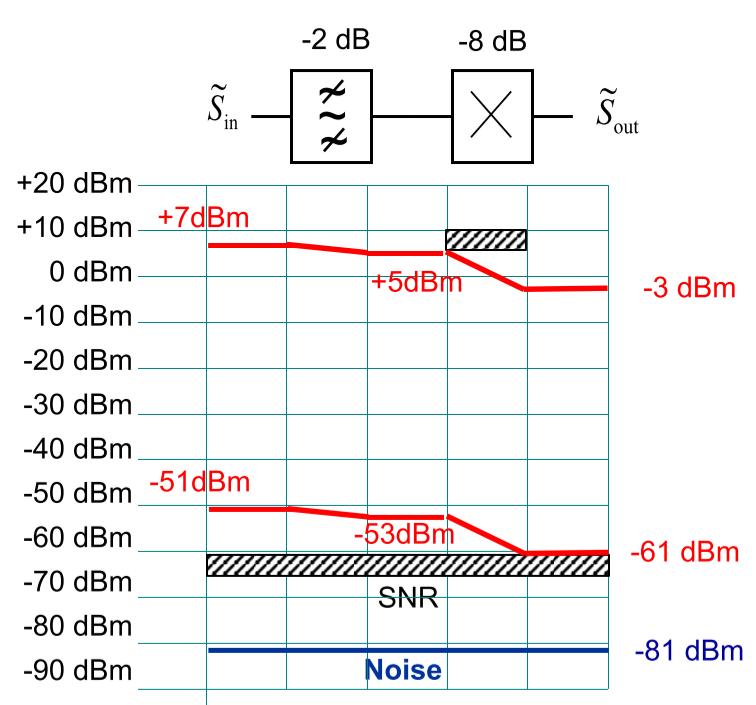
\includegraphics[width=.9\linewidth]{./06-leitungscodierung/hs2018}
    \vspace{-8pt}
\end{center}

\subsubsection{Prüfung HS2016}
Eine Datenquelle sendet dauernd die Einersequenz $'....1 1 1 1 1 1 ...'$. Kreuzen Sie an, ob die unten aufgeführten Leitungscodes für diese Sequenz annähernd gleichspannungsfrei sind, res-
pektive ob genügend Pegelwechsel für eine Taktrückgewinnung vorhanden sind.
\begin{center}
    \vspace{-8pt}
    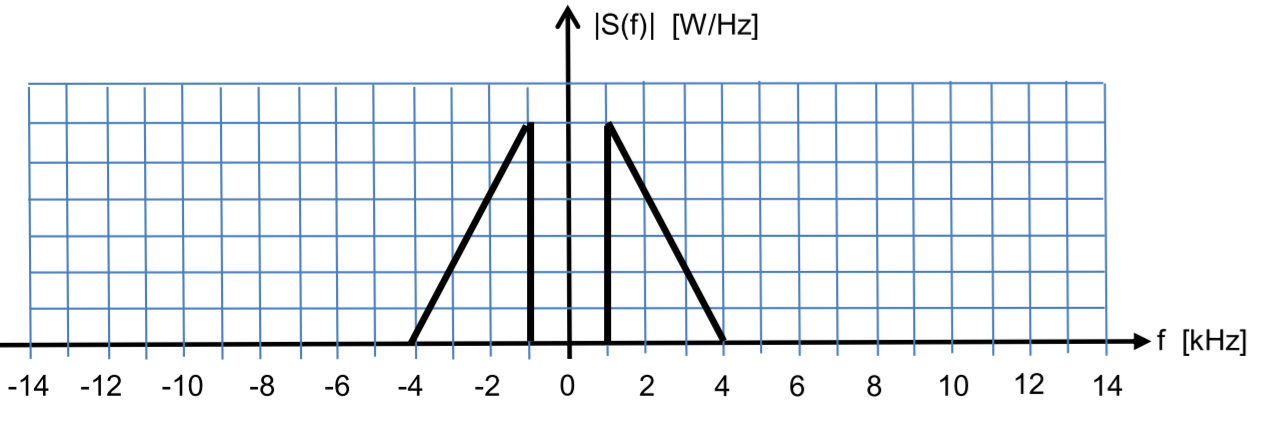
\includegraphics[width=.9\linewidth]{./06-leitungscodierung/hs2016}
    \vspace{-8pt}
\end{center}
